%!TEX root = ../thesis.tex
% **************************** Define Graphics Path **************************
\ifpdf
\graphicspath{{Chapter5/Figs/Raster/}{Chapter5/Figs/PDF/}{Chapter5/Figs/}}
\else
\graphicspath{{Chapter5/Figs/Vector/}{Chapter5/Figs/}}
\fi

%*******************************************************************************
%****************************** Fifth Chapter *********************************
%*******************************************************************************

\chapter{Experiments and Results}
\label{chapter5}

\section{Training the rates}
\subsection{The elusive timescale $\lambda$}
\begin{figure}[H]
	\centering
	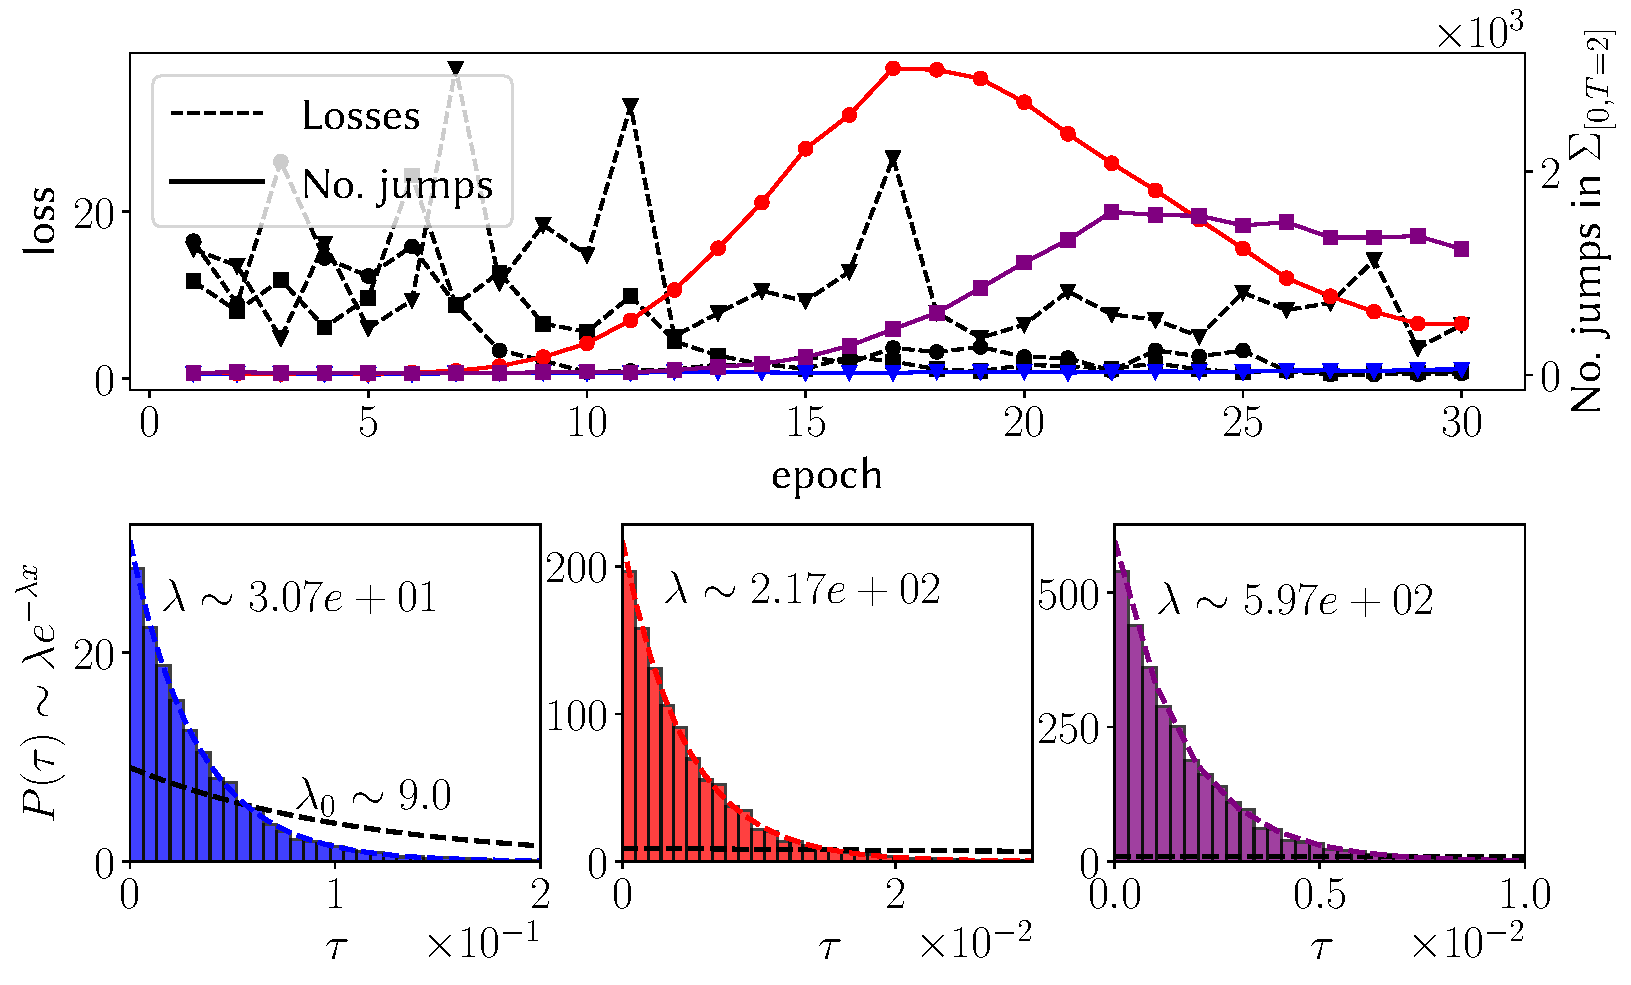
\includegraphics[width=\linewidth]{Chapter5/Figs/Vector/scale_blowup}
	\caption[The inability of the method to learn the correct time scale $\lambda$]{\textbf{The inability of the method to learn the correct time scale $\lambda$.}}
	\label{fig:scaleblowup}
\end{figure}

\begin{figure}[H]
	\centering
	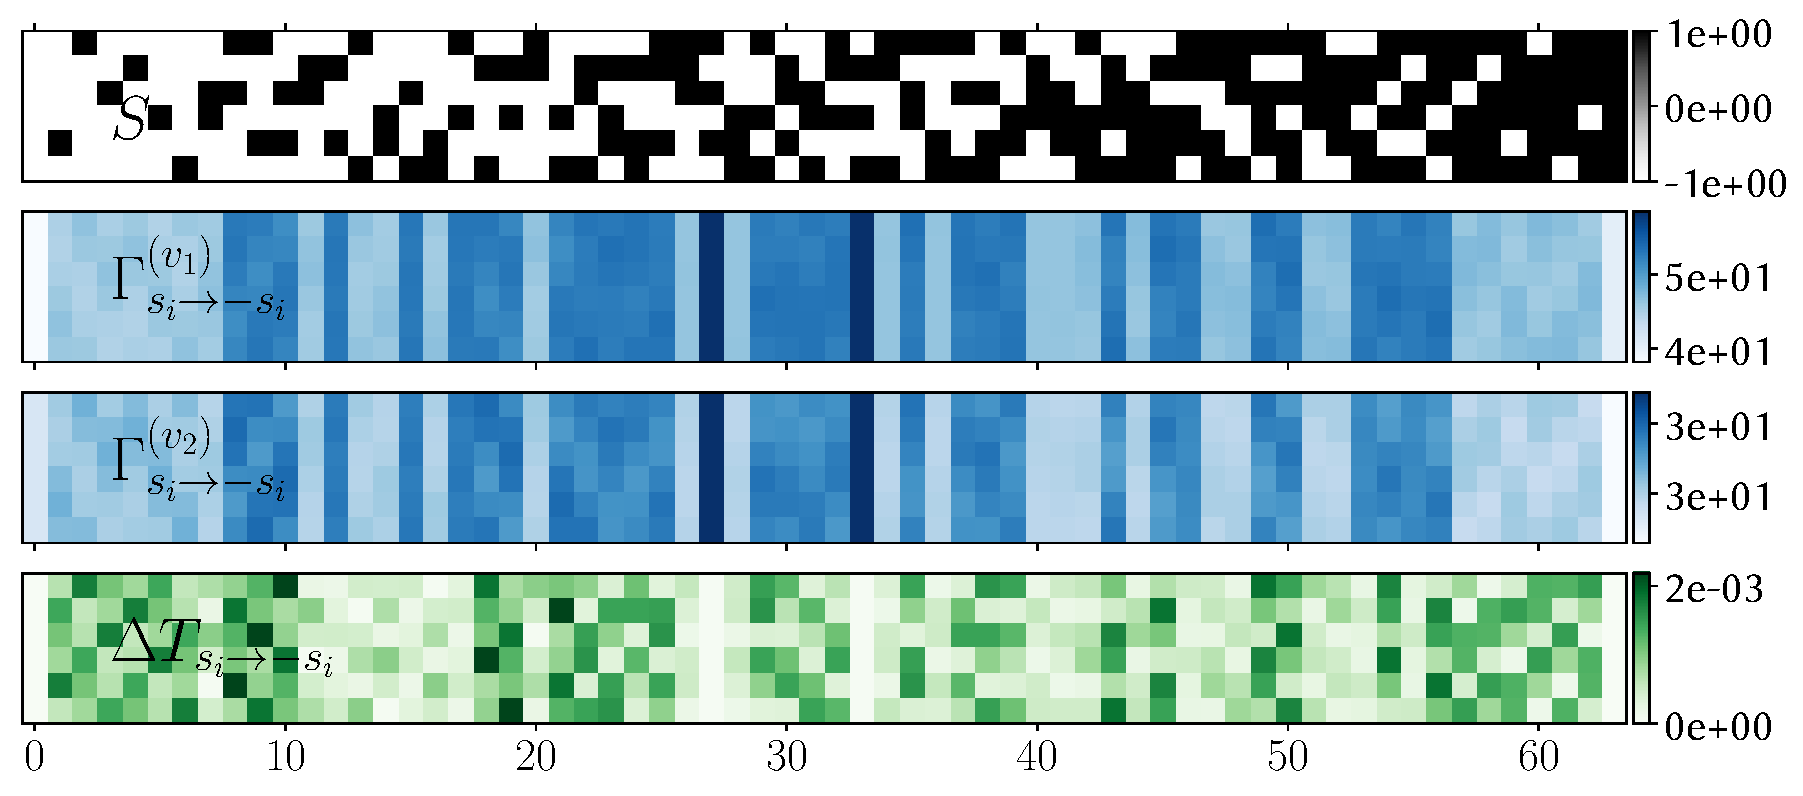
\includegraphics[width=\linewidth]{Chapter5/Figs/Vector/rate_structure.pdf}
	\caption[Structure of learned rates for 1D TFIM]{\textbf{Structure of rates in 1D TFIM.}}
	\label{fig:}
\end{figure}

\subsubsection{What can we do about this?}

\subsection{Architectural choices}
\begin{figure}[H]
	\centering
	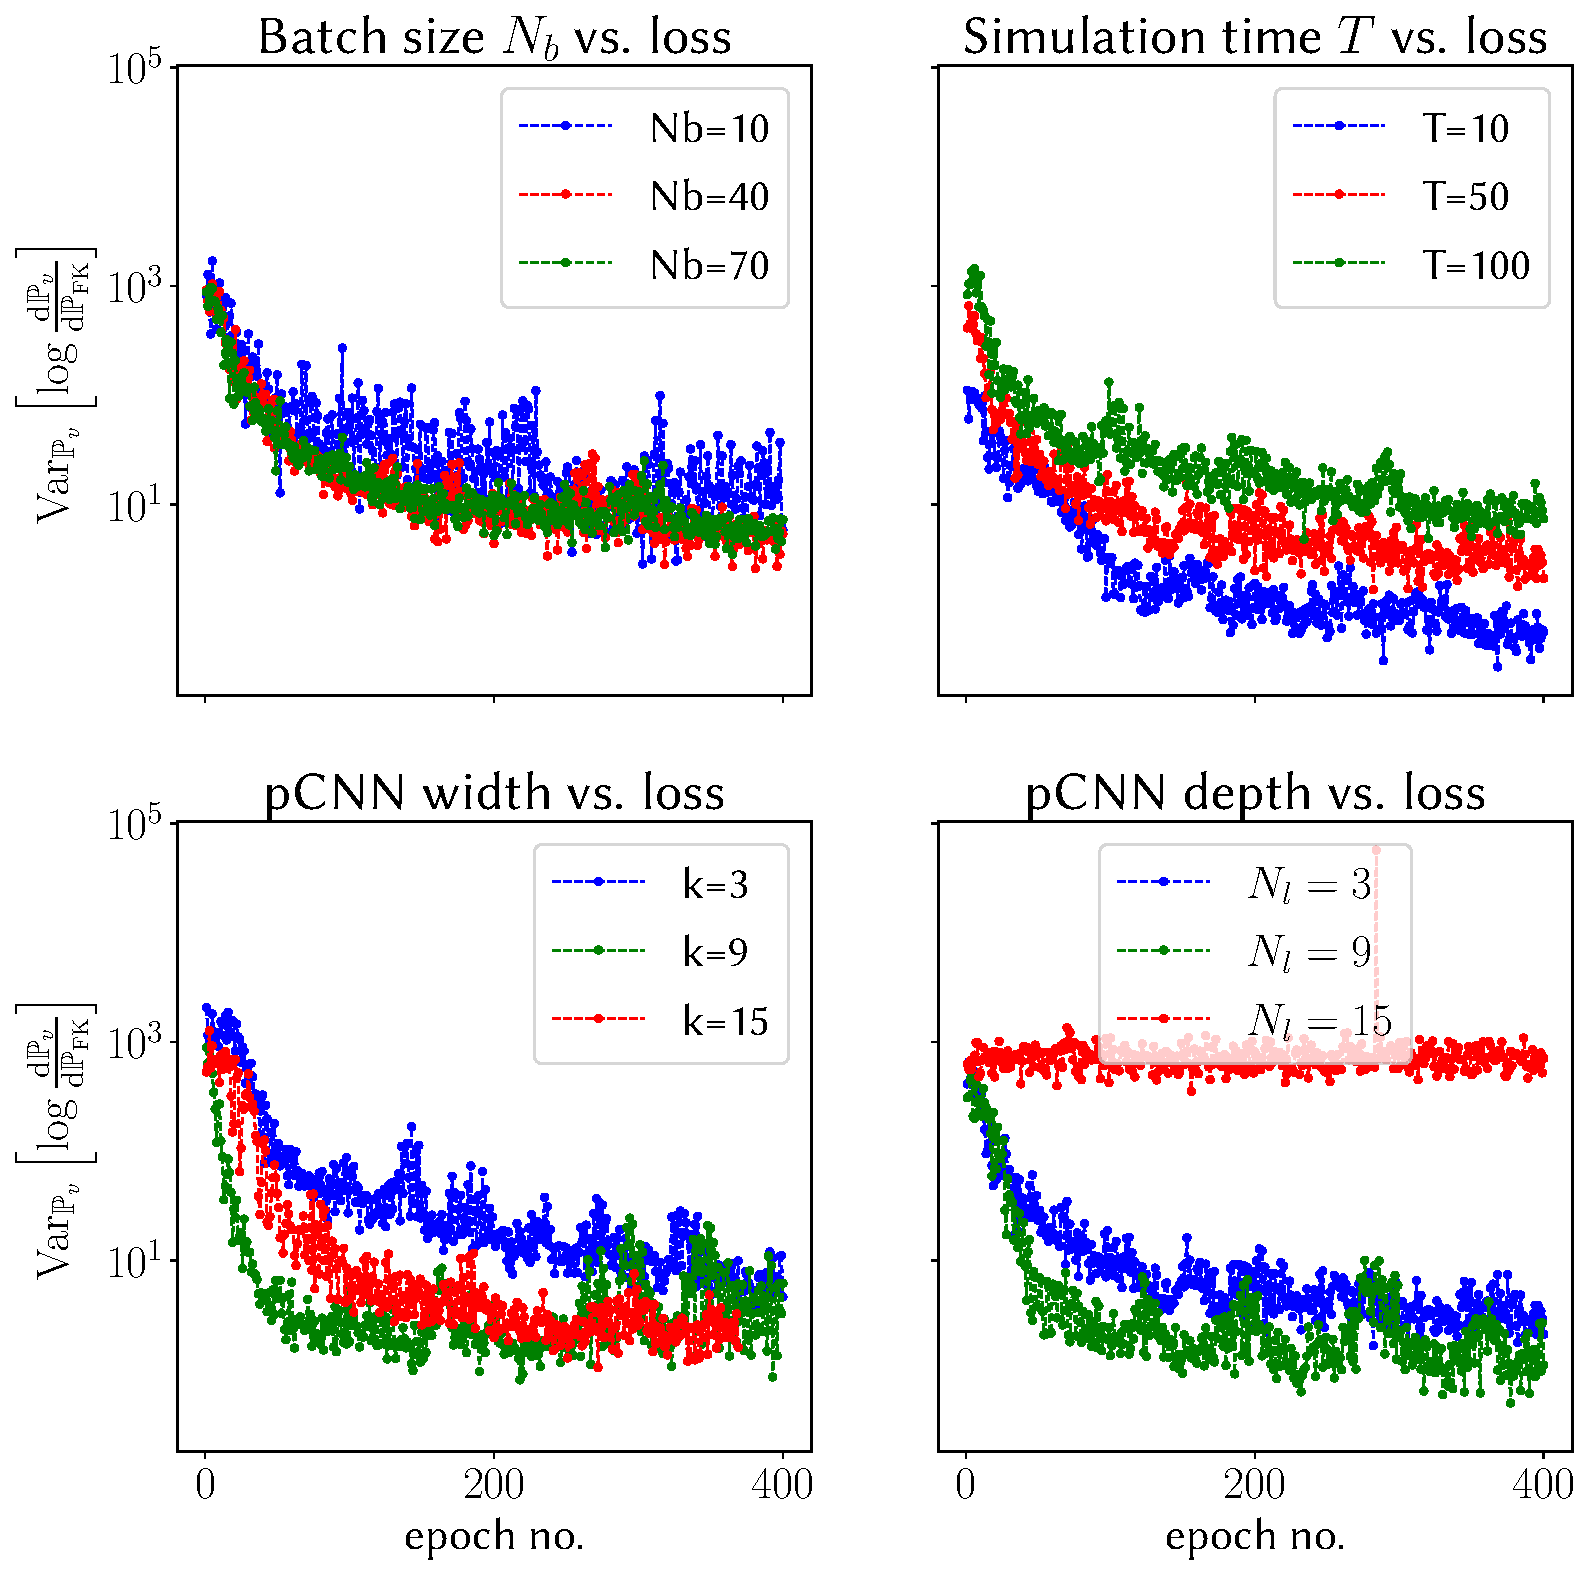
\includegraphics[width=\linewidth]{Chapter5/Figs/Vector/init_test_learning}
	\caption[Initial rate training experiments]{\textbf{Initial rate training experiments}}
	\label{fig:inittestlearning}
\end{figure}

\begin{figure}[H]
	\centering
	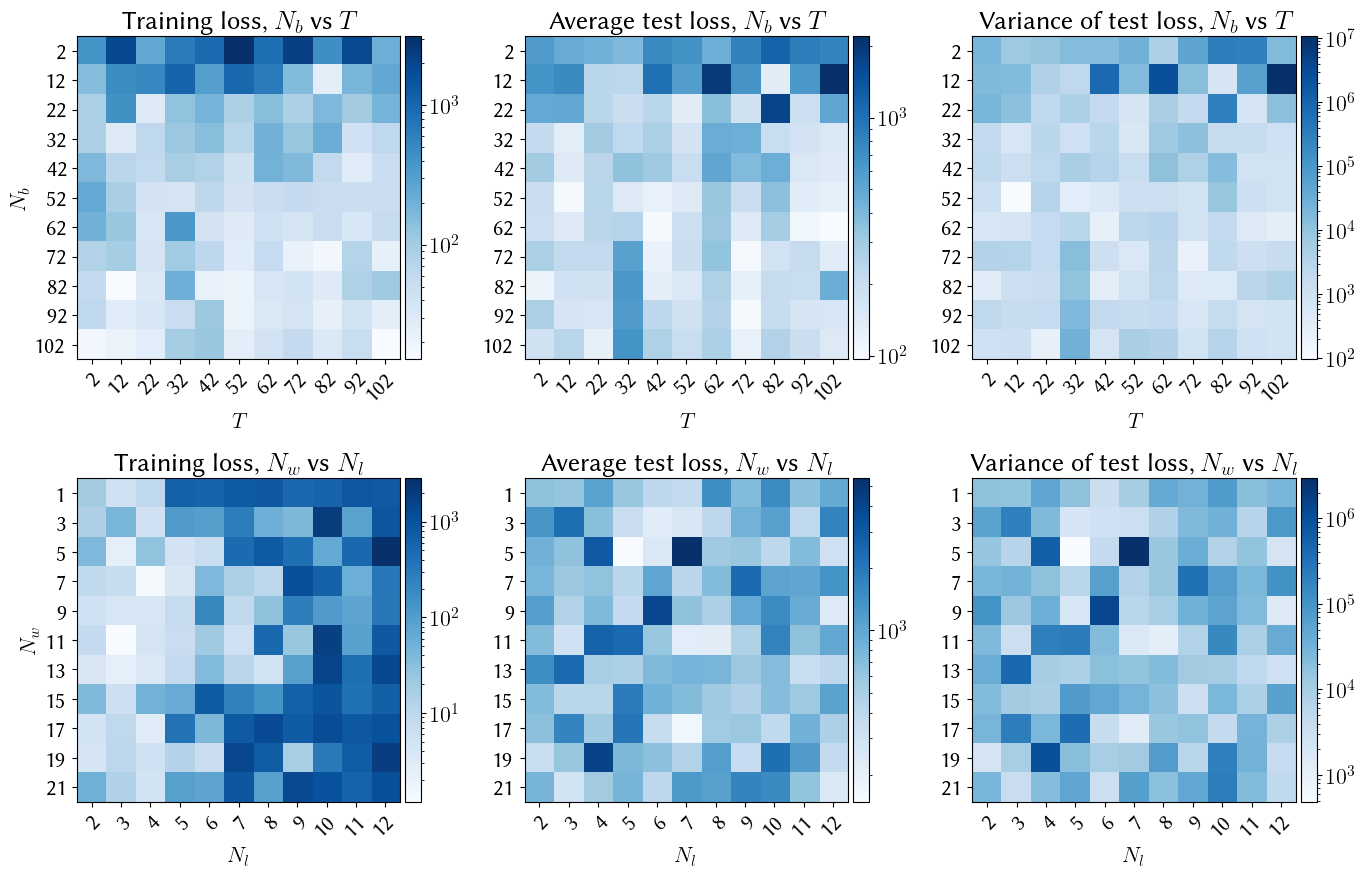
\includegraphics[width=\linewidth]{Chapter5/Figs/Raster/avg_var_loss}
	\caption[Performance of the pCNN for different setups]{\textbf{Performance of the pCNN for different setups.}}
	\label{fig:avgvarloss}
\end{figure}

\begin{figure}[H]
	\centering
	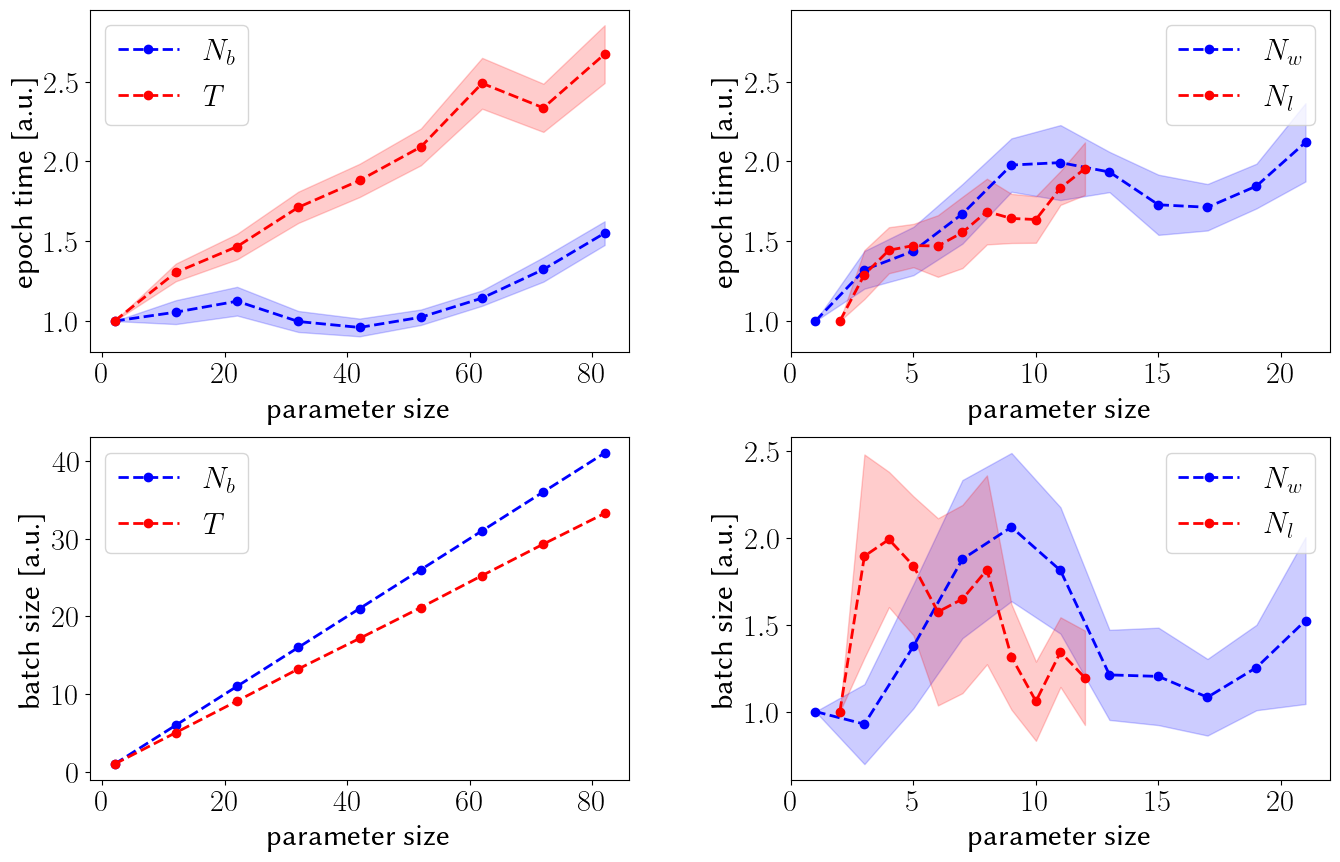
\includegraphics[width=\linewidth]{Chapter5/Figs/Raster/initial_time_space}
	\caption[Time and space complexity of the pCNN]{\textbf{Time and space complexity of the pCNN}}
	\label{fig:initialtimespace}
\end{figure}


\section{Importance sampling}
\section{Results}
\subsection{Ising model}
\subsubsection{One dimension}
\subsubsection{Two dimensions}
\subsection{XY model}